% quarto_capitolo.tex

\chapter{Metodi di risoluzione delle reti}

\begin{concetto}
Nei capitoli precedenti abbiamo imparato a conoscere i componenti fondamentali di un circuito e le due leggi di Kirchhoff. Applicando queste leggi a un circuito semplice, con una sola maglia o con pochi nodi, la soluzione si ottiene con pochi passaggi. Quando però il circuito diventa più complesso, con più generatori e più maglie, il numero di equazioni da scrivere cresce rapidamente e la risoluzione diretta diventa laboriosa.

In questo capitolo introduciamo alcuni \textbf{metodi di risoluzione} che permettono di semplificare il problema. Alcuni riducono il numero di equazioni da scrivere, altri trasformano una rete complessa in una rete equivalente più semplice. L'obiettivo non è sostituire le leggi di Kirchhoff, ma usarle in modo più intelligente.
\end{concetto}

\section{Il metodo delle correnti di maglia}

\begin{concetto}
Il \textbf{metodo delle correnti di maglia} consiste nell'associare a ogni maglia elementare del circuito una \textbf{corrente fittizia} che la percorre in senso chiuso. Le correnti reali dei rami si ottengono poi come combinazione algebrica delle correnti di maglia.
\end{concetto}

L'idea alla base del metodo è semplice: invece di scrivere un'equazione per ogni ramo del circuito, si scrive \textbf{un'equazione per ogni maglia elementare}. In questo modo il numero di equazioni è pari al numero di maglie, che è generalmente inferiore al numero di rami.

\subsection{La procedura}

La procedura per applicare il metodo delle correnti di maglia è la seguente:

\begin{enumerate}[leftmargin=1cm]
  \item si individuano tutte le \textbf{maglie elementari} del circuito;
  \item si assegna a ciascuna maglia una \textbf{corrente di maglia} \(i_1, i_2, \dots\), scegliendo arbitrariamente un verso di percorrenza (di solito tutte nello stesso verso, per esempio orario);
  \item si scrive per ogni maglia la \textbf{legge di Kirchhoff alle tensioni}, esprimendo le cadute di tensione sui resistori in funzione delle correnti di maglia;
  \item si risolve il sistema di equazioni così ottenuto, trovando i valori delle correnti di maglia;
  \item si ricavano le \textbf{correnti reali dei rami} sommando algebricamente le correnti di maglia che attraversano quel ramo.
\end{enumerate}

\begin{attenzione}
La corrente di maglia non è una corrente fisica: è un artificio di calcolo. Solo le correnti dei rami hanno un significato fisico. In un ramo percorso da più correnti di maglia, la corrente reale è la somma algebrica di esse.
\end{attenzione}

\subsection{Esempio di applicazione}

\begin{esempio}
\textbf{Circuito con due maglie.}  Vogliamo calcolare le correnti che attraversano i rami.

\begin{center}
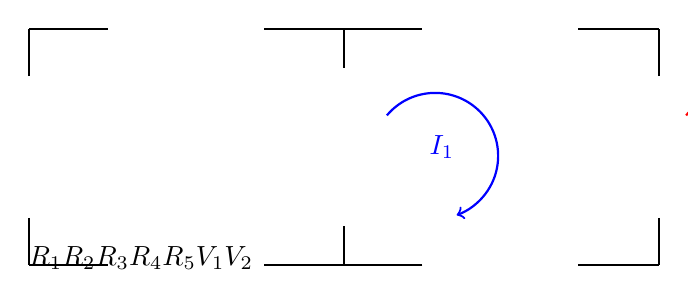
\begin{tikzpicture}[scale=1]
  % Nodi
  \coordinate (A) at (0,0);
  \coordinate (B) at (4,0);
  \coordinate (C) at (0,3);
  \coordinate (D) at (4,3);
  \coordinate (E) at (8,3);
  \coordinate (F) at (8,0);

  % Rami
  \draw[thick] (A) -- (1, 0);
  \draw[thick] (B) -- (2.99, 0);
  \draw[thick] (B) -- (4, 0.5);
  \draw[thick] (D) -- (4, 2.5);
  \draw[thick] (1, 3) -- (C);
  \draw[thick] (2.99, 3) -- (D);
  \draw[thick] (0, 0.6) -- (A);
  \draw[thick] (0, 2.4) -- (C);
  \draw[thick] (D) -- (5, 3);
  \draw[thick] (6.98, 3) -- (E);
  \draw[thick] (8, 2.4) -- (E);
  \draw[thick] (8, 0.6) -- (F);
  \draw[thick] (6.98, 0) -- (F);
  \draw[thick] (5, 0) -- (B);


  % Componenti
  \resistoreANSI[rot=0, label=$R_1$, label dy=0.5]{2}{0}{}
  \resistoreANSI[rot=90, label=$R_2$, label dx=0.5, label dy=0]{4}{1.5}{}
  \resistoreANSI[rot=0, label=$R_3$, label dy=-0.5]{2}{3}{}
  \resistoreANSI[rot=0, label=$R_4$, label dy=-0.5]{6}{3}{}
  \resistoreANSI[rot=0, label=$R_5$, label dy=0.5]{6}{0}{}
  \generatore[rot=0, label = $V_1$, label dx = 0.8]{0}{1.5}
  \generatore[rot=0, label = $V_2$, label dx = -0.7]{8}{1.5}

  % Correnti di maglia
  \draw[->, thick, blue] (1.7,1.9) arc (140:-70:0.8);
  \node[blue] at (2.4,1.5) {$I_1$};
  \draw[->, thick, red] (5.5,1.9) arc (140:-70:0.8);
  \node[red] at (6.2,1.5) {$I_2$};
\end{tikzpicture}
\end{center}

\textbf{Soluzione.} Individuiamo due maglie elementari: la maglia di sinistra (percorsa da \(I_1\) in senso orario) e la maglia di destra (percorsa da \(I_2\) in senso orario).

Per la maglia di sinistra, applicando la LKT:
\[
V_1 - R_1 I_1 - R_3 I_1 - R_2 I_1 + R_2 I_2 = 0.
\]
Il termine \(+R_2 I_2\) tiene conto del fatto che il resistore \(R_2\) è percorso anche da \(I_2\) con verso opposto rispetto a \(I_1\).

Per la maglia di destra:
\[
-V_2 - R_4 I_2 - R_5 I_2 - R_2 I_2 + R_2 I_1 = 0.
\]

Raccogliendo i termini:
\[
\begin{cases}
(R_1 + R_3 + R_2)\,I_1 - R_2\,I_2 = V_1 \\
-R_2\,I_1 + (R_4 + R_5 + R_2)\,I_2 = -V_2
\end{cases}
\]

Con valori numerici \(R_1 = 1\,\Omega\), \(R_2 = 3\,\Omega\), \(R_3 = 1\,\Omega\), \(R_4 = 1\,\Omega\), \(R_5 = 1\,\Omega\), \(V_1 = 10\,\text{V}\), \(V_2 = 4\,\text{V}\):
\[
\begin{cases}
5\,I_1 - 3\,I_2 = 10 \\
-3\,I_1 + 5\,I_2 = -4
\end{cases}
\]

Risolvendo il sistema, troviamo i valori delle due correnti fittizie:
\[
I_1 = 2{,}375\,\text{A} \qquad I_2 = 0{,}625\,\text{A}.
\]
La corrente nel ramo centrale (percorso da \(R_2\)) è la differenza tra le due correnti di maglia:
\[
I_{R_2} = I_1 - I_2 = 2{,}375 - 0{,}625 = 1{,}75\,\text{A}.
\]
\end{esempio}

\section{Il principio di sovrapposizione degli effetti}

\begin{concetto}
Il \textbf{principio di sovrapposizione degli effetti} afferma che in un circuito lineare con più generatori, la corrente (o la tensione) in un qualsiasi ramo è la \textbf{somma algebrica} degli effetti prodotti da ciascun generatore considerato singolarmente, con tutti gli altri generatori spenti.
\end{concetto}

Spegnere un generatore significa:
\begin{itemize}[leftmargin=1cm]
  \item sostituire un \textbf{generatore di tensione} con un \textbf{corto circuito};
  \item sostituire un \textbf{generatore di corrente} con un \textbf{circuito aperto}.
\end{itemize}

\subsection{La procedura}

\begin{enumerate}[leftmargin=1cm]
  \item si considera acceso un solo generatore alla volta, spegnendo tutti gli altri;
  \item per ogni generatore, si calcola la corrente (o la tensione) richiesta nel ramo di interesse;
  \item si sommano algebricamente i contributi di tutti i generatori, tenendo conto dei versi.
\end{enumerate}

\begin{attenzione}
Il principio di sovrapposizione vale solo per circuiti \textbf{lineari}, cioè quelli in cui la relazione tra tensione e corrente è lineare (come la legge di Ohm). Non vale per componenti non lineari come diodi o transistor.
\end{attenzione}



\begin{esempio}
\textbf{Circuito con due maglie risolto con la sovrapposizione degli effetti.} 
Riprendiamo lo stesso circuito dell'esempio precedente: due maglie, cinque resistori e due generatori. Vogliamo calcolare la corrente nel ramo centrale (quello percorso da \(R_2\)) usando il principio di sovrapposizione degli effetti.

\begin{center}
\begin{tikzpicture}[scale=1]
  \coordinate (A) at (0,0);
  \coordinate (B) at (4,0);
  \coordinate (C) at (0,3);
  \coordinate (D) at (4,3);
  \coordinate (E) at (8,3);
  \coordinate (F) at (8,0);

  \draw[thick] (A) -- (1, 0);
  \draw[thick] (B) -- (2.99, 0);
  \draw[thick] (B) -- (4, 0.5);
  \draw[thick] (D) -- (4, 2.5);
  \draw[thick] (1, 3) -- (C);
  \draw[thick] (2.99, 3) -- (D);
  \draw[thick] (0, 0.6) -- (A);
  \draw[thick] (0, 2.4) -- (C);
  \draw[thick] (D) -- (5, 3);
  \draw[thick] (6.98, 3) -- (E);
  \draw[thick] (8, 2.4) -- (E);
  \draw[thick] (8, 0.6) -- (F);
  \draw[thick] (6.98, 0) -- (F);
  \draw[thick] (5, 0) -- (B);

  \resistoreANSI[rot=0, label=$R_1$, label dy=0.5]{2}{0}
  \resistoreANSI[rot=90, label=$R_2$, label dx=0.5, label dy=0]{4}{1.5}
  \resistoreANSI[rot=0, label=$R_3$, label dy=-0.5]{2}{3}
  \resistoreANSI[rot=0, label=$R_4$, label dy=-0.5]{6}{3}
  \resistoreANSI[rot=0, label=$R_5$, label dy=0.5]{6}{0}
  \generatore[rot=0, label=$V_1$, label dx=0.8]{0}{1.5}
  \generatore[rot=0, label=$V_2$, label dx=-0.7]{8}{1.5}
\end{tikzpicture}
\end{center}

\textbf{Procedura.} Il principio di sovrapposizione degli effetti si applica in tre passi:
\begin{enumerate}[leftmargin=1cm]
  \item si spegne \(V_2\) (sostituendolo con un corto circuito) e si calcola il contributo di \(V_1\) da solo;
  \item si spegne \(V_1\) (sostituendolo con un corto circuito) e si calcola il contributo di \(V_2\) da solo;
  \item si sommano algebricamente i due contributi per ottenere la corrente reale.
\end{enumerate}

I valori numerici sono: \(R_1 = 1\,\Omega\), \(R_2 = 3\,\Omega\), \(R_3 = 1\,\Omega\), \(R_4 = 1\,\Omega\), \(R_5 = 1\,\Omega\), \(V_1 = 10\,\text{V}\), \(V_2 = 4\,\text{V}\).

\subsubsection*{Passo 1: acceso solo \(V_1\)}

Spegniamo \(V_2\) sostituendolo con un filo (corto circuito). Il circuito diventa:

\begin{center}
\begin{tikzpicture}[scale=1]
  \coordinate (A) at (0,0);
  \coordinate (B) at (4,0);
  \coordinate (C) at (0,3);
  \coordinate (D) at (4,3);
  \coordinate (E) at (8,3);
  \coordinate (F) at (8,0);

  \draw[thick] (A) -- (1, 0);
  \draw[thick] (B) -- (2.99, 0);
  \draw[thick] (B) -- (4, 0.5);
  \draw[thick] (D) -- (4, 2.5);
  \draw[thick] (1, 3) -- (C);
  \draw[thick] (2.99, 3) -- (D);
  \draw[thick] (0, 0.6) -- (A);
  \draw[thick] (0, 2.4) -- (C);
  \draw[thick] (D) -- (5, 3);
  \draw[thick] (6.98, 3) -- (E);
  \draw[thick] (8, 3) -- (8, 0);
  \draw[thick] (6.98, 0) -- (F);
  \draw[thick] (5, 0) -- (B);

  \resistoreANSI[rot=0, label=$R_1$, label dy=0.5]{2}{0}
  \resistoreANSI[rot=90, label=$R_2$, label dx=0.5, label dy=0]{4}{1.5}
  \resistoreANSI[rot=0, label=$R_3$, label dy=-0.5]{2}{3}
  \resistoreANSI[rot=0, label=$R_4$, label dy=-0.5]{6}{3}
  \resistoreANSI[rot=0, label=$R_5$, label dy=0.5]{6}{0}
  \generatore[rot=0, label=$V_1$, label dx=0.8]{0}{1.5}
\end{tikzpicture}
\end{center}

Con \(V_2\) spento, il resistore \(R_5\) viene collegato direttamente al nodo inferiore destro e il resistore \(R_4\) al nodo superiore destro, entrambi in parallelo al ramo di \(R_2\).

Possiamo procedere in due modi: o ridurre il circuito, oppure applicare direttamente il partitore di tensione. Vediamo il metodo della riduzione.

Il ramo di destra, formato da \(R_4\) e \(R_5\) in serie, ha resistenza:
\[
R_{45} = R_4 + R_5 = 1 + 1 = 2\,\Omega.
\]

Questo ramo è in parallelo a \(R_2\), quindi la resistenza equivalente del parallelo è:
\[
R_{2,45} = \frac{R_2 \cdot R_{45}}{R_2 + R_{45}} = \frac{3 \cdot 2}{3 + 2} = \frac{6}{5} = 1{,}2\,\Omega.
\]

\begin{center}
\begin{tikzpicture}[scale=1]
  \coordinate (A) at (0,0);
  \coordinate (B) at (4,0);
  \coordinate (C) at (0,3);
  \coordinate (D) at (4,3);

  \draw[thick] (A) -- (1, 0);
  \draw[thick] (B) -- (2.99, 0);
  \draw[thick] (B) -- (4, 0.5);
  \draw[thick] (D) -- (4, 2.5);
  \draw[thick] (1, 3) -- (C);
  \draw[thick] (2.99, 3) -- (D);
  \draw[thick] (0, 0.6) -- (A);
  \draw[thick] (0, 2.4) -- (C);

  \resistoreANSI[rot=0, label=$R_1$, label dy=0.5]{2}{0}
  \resistoreANSI[rot=90, label=$R_{2,45}$, label dx=0.7, label dy=0]{4}{1.5}
  \resistoreANSI[rot=0, label=$R_3$, label dy=-0.5]{2}{3}
  \generatore[rot=0, label=$V_1$, label dx=0.8]{0}{1.5}
\end{tikzpicture}
\end{center}

Ora il circuito è una maglia unica formata da \(V_1\), \(R_1\), \(R_3\) e \(R_{2,45}\) in serie. La resistenza totale è:
\[
R_{\text{tot}}^{(1)} = R_1 + R_3 + R_{2,45} = 1 + 1 + 1{,}2 = 3{,}2\,\Omega.
\]

La corrente totale che circola nel circuito è:
\[
I_{\text{tot}}^{(1)} = \frac{V_1}{R_{\text{tot}}^{(1)}} = \frac{10}{3{,}2} = 3{,}125\,\text{A}.
\]

Questa corrente passa attraverso \(R_1\) e \(R_3\), poi arriva al parallelo \(R_2 \parallel R_{45}\) e si ripartisce. La corrente che attraversa \(R_2\) si calcola con il partitore di corrente:
\[
I_{R_2}^{(1)} = I_{\text{tot}}^{(1)} \cdot \frac{R_{45}}{R_2 + R_{45}} = 3{,}125 \cdot \frac{2}{3 + 2} = 3{,}125 \cdot 0{,}4 = 1{,}25\,\text{A}.
\]

Quindi il contributo di \(V_1\) alla corrente in \(R_2\) è:
\[
I_{R_2}^{(1)} = 1{,}25\,\text{A},
\]
diretta dall'alto verso il basso (cioè dal nodo superiore a quello inferiore).

\subsubsection*{Passo 2: acceso solo \(V_2\)}

Spegniamo \(V_1\) sostituendolo con un filo (corto circuito). Il circuito diventa:

\begin{center}
\begin{tikzpicture}[scale=1]
  \coordinate (A) at (0,0);
  \coordinate (B) at (4,0);
  \coordinate (C) at (0,3);
  \coordinate (D) at (4,3);
  \coordinate (E) at (8,3);
  \coordinate (F) at (8,0);

  \draw[thick] (A) -- (1, 0);
  \draw[thick] (B) -- (2.99, 0);
  \draw[thick] (B) -- (4, 0.5);
  \draw[thick] (D) -- (4, 2.5);
  \draw[thick] (1, 3) -- (C);
  \draw[thick] (2.99, 3) -- (D);
  \draw[thick] (0, 3) -- (0, 0);
  \draw[thick] (D) -- (5, 3);
  \draw[thick] (6.98, 3) -- (E);
  \draw[thick] (8, 2.4) -- (E);
  \draw[thick] (8, 0.6) -- (F);
  \draw[thick] (6.98, 0) -- (F);
  \draw[thick] (5, 0) -- (B);

  \resistoreANSI[rot=0, label=$R_1$, label dy=0.5]{2}{0}
  \resistoreANSI[rot=90, label=$R_2$, label dx=0.5, label dy=0]{4}{1.5}
  \resistoreANSI[rot=0, label=$R_3$, label dy=-0.5]{2}{3}
  \resistoreANSI[rot=0, label=$R_4$, label dy=-0.5]{6}{3}
  \resistoreANSI[rot=0, label=$R_5$, label dy=0.5]{6}{0}
  \generatore[rot=0, label=$V_2$, label dx=-0.7]{8}{1.5}
\end{tikzpicture}
\end{center}

Con \(V_1\) spento, il resistore \(R_1\) viene collegato direttamente al nodo inferiore sinistro e il resistore \(R_3\) al nodo superiore sinistro, entrambi in parallelo al ramo di \(R_2\).

Il ramo di sinistra, formato da \(R_1\) e \(R_3\) in serie, ha resistenza:
\[
R_{13} = R_1 + R_3 = 1 + 1 = 2\,\Omega.
\]

Questo ramo è in parallelo a \(R_2\), quindi la resistenza equivalente del parallelo è:
\[
R_{2,13} = \frac{R_2 \cdot R_{13}}{R_2 + R_{13}} = \frac{3 \cdot 2}{3 + 2} = \frac{6}{5} = 1{,}2\,\Omega.
\]

Ora il circuito è una maglia unica formata da \(V_2\), \(R_4\), \(R_5\) e \(R_{2,13}\) in serie. La resistenza totale è:
\[
R_{\text{tot}}^{(2)} = R_4 + R_5 + R_{2,13} = 1 + 1 + 1{,}2 = 3{,}2\,\Omega.
\]

La corrente totale che circola nel circuito è:
\[
I_{\text{tot}}^{(2)} = \frac{V_2}{R_{\text{tot}}^{(2)}} = \frac{4}{3{,}2} = 1{,}25\,\text{A}.
\]

Questa corrente passa attraverso \(R_4\) e \(R_5\), poi arriva al parallelo \(R_2 \parallel R_{13}\) e si ripartisce. La corrente che attraversa \(R_2\) si calcola con il partitore di corrente:
\[
I_{R_2}^{(2)} = I_{\text{tot}}^{(2)} \cdot \frac{R_{13}}{R_2 + R_{13}} = 1{,}25 \cdot \frac{2}{3 + 2} = 1{,}25 \cdot 0{,}4 = 0{,}5\,\text{A}.
\]

Quindi il contributo di \(V_2\) alla corrente in \(R_2\) è:
\[
I_{R_2}^{(2)} = 0{,}5\,\text{A}.
\]

\subsubsection*{Passo 3: somma dei contributi}

I due contributi hanno \textbf{verso concorde} nel ramo centrale:
\begin{itemize}[leftmargin=1cm]
  \item \(I_{R_2}^{(1)} = 1{,}25\,\text{A}\) diretto dall'alto verso il basso;
  \item \(I_{R_2}^{(2)} = 0{,}5\,\text{A}\) diretto dall'alto verso il basso.
\end{itemize}

Prendiamo come verso positivo quello dall'alto verso il basso. Allora:
\[
I_{R_2} = I_{R_2}^{(1)} + I_{R_2}^{(2)} = 1{,}25 + 0{,}5 = 1{,}75\,\text{A}.
\]

La corrente nel ramo centrale è quindi \(0{,}75\,\text{A}\), diretta dall'alto verso il basso.

\end{esempio}




















\section{Il teorema di Thévenin}

\begin{concetto}
Il \textbf{teorema di Thévenin} afferma che qualsiasi rete lineare, vista da due terminali A e B, può essere sostituita da un \textbf{circuito equivalente} formato da un solo generatore di tensione \(V_{Th}\) in serie con un solo resistore \(R_{Th}\).
\end{concetto}

I due parametri del circuito equivalente si calcolano così:
\begin{itemize}[leftmargin=1cm]
  \item \(V_{Th}\) è la \textbf{tensione a vuoto} tra i terminali A e B, cioè la tensione misurata quando non è collegato alcun carico;
  \item \(R_{Th}\) è la \textbf{resistenza equivalente} vista dai terminali A e B, calcolata spegnendo tutti i generatori indipendenti (generatori di tensione cortocircuitati, generatori di corrente aperti).
\end{itemize}

\begin{center}
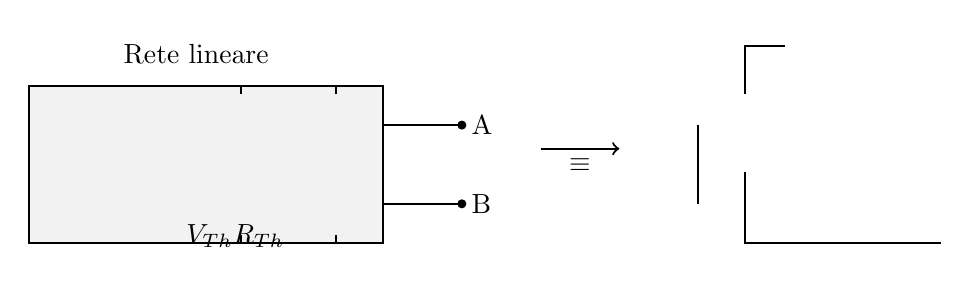
\begin{tikzpicture}[scale=1]
  % Rete originale
  \draw[thick, fill=gray!10] (-2,0) rectangle (2.5,2);
  \node at (0.125,2.4) {Rete lineare};
  \draw[thick] (2.5,1.5) -- (3.5,1.5);
  \draw[thick] (2.5,0.5) -- (3.5,0.5);
  \resistoreANSI[rot=90]{-1.6}{1}{}
  \resistoreANSI[rot=90]{-1}{1}{}
  \resistoreANSI[rot=90]{-0.4}{1}{}
  \generatore[rot=0]{0.7}{1}{}
  \draw[thick] (0.7,0) -- (0.7,0.11);
  \draw[thick] (1.9,0) -- (1.9,0.11);
  \draw[thick] (0.7,1.89) -- (0.7,2);
  \draw[thick] (1.9,1.89) -- (1.9,2);
  \generatore[rot=180]{1.9}{1}{}


  \filldraw (3.5,1.5) circle (0.05) node[right] {A};
  \filldraw (3.5,0.5) circle (0.05) node[right] {B};

  % Freccia di equivalenza
  \draw[->, thick] (4.5,1.2) -- (5.5,1.2) node[midway,below] {\(\equiv\)};

  % Circuito equivalente di Thévenin
  \draw[thick] (6.5,0.5) -- (6.5,1.5);
  \generatore[rot=0, label=$V_{Th}$, label dx=0.85, label dy=0]{6.5}{1}{}
  \draw[thick] (6.5,1.9) -- (6.5,2.5) -- (7.01, 2.5);
  \draw[thick] (6.5,0.9) -- (6.5,0) -- (9, 0);
  \resistoreANSI[rot=0, label=$R_{Th}$, label dy=0.5]{8}{2.5}{}
  
  \filldraw (9,2.5) circle (0.05) node[right] {A};
  \filldraw (9,0) circle (0.05) node[right] {B};
\end{tikzpicture}
\end{center}

\begin{esempio}
\textbf{Calcolo del circuito equivalente.} Si consideri il circuito usato negli esempi precedenti. Vogliamo il circuito equivalente di Thévenin visto ai capi di \(R_2\). Ridisegnamo il circuito per capire meglio dove poter identificare la porta AB:




\begin{center}
\begin{tikzpicture}[scale=1]
  \coordinate (A) at (0,0);
  \coordinate (B) at (4,0);
  \coordinate (C) at (0,6);
  \coordinate (D) at (4,6);
  \coordinate (E) at (8,6);
  \coordinate (F) at (8,0);

  % Rami orizzontali
  \draw[thick] (A) -- (1, 0);
  \draw[thick] (B) -- (2.99, 0);
  \draw[thick] (1, 6) -- (C);
  \draw[thick] (2.99, 6) -- (D);
  \draw[thick] (0, 2.4) -- (A);
  \draw[thick] (0, 3.89) -- (C);
  \draw[thick] (8, 4) -- (E);
  \draw[thick] (8, 2.01) -- (F);
  \draw[thick] (B) -- (F);
  \draw[thick] (D) -- (E);
  
  \draw[thick] (4, 2) -- (4, 2.1);
  \draw[thick] (4, 3.9) -- (4, 4);

  % Ramo centrale: R4, R5 e V2
  \resistoreANSI[rot=90, label=$R_4$, label dx=0.6, label dy=0]{4}{5}
  \resistoreANSI[rot=90, label=$R_5$, label dx=0.6, label dy=0]{4}{1}
  \generatore[rot=0, label=$V_2$, label dx=0.7, label dy=0]{4}{3}

  % Componenti sugli altri rami
  \resistoreANSI[rot=0, label=$R_1$, label dy=0.5]{2}{0}
  \resistoreANSI[rot=0, label=$R_3$, label dy=-0.5]{2}{6}
  \generatore[rot=0, label=$V_1$, label dx=0.8]{0}{3}

  % R2 sul ramo destro
  \resistoreANSI[rot=90, label=$R_2$, label dx=0.6, label dy=0]{8}{3}

  % Porta AB ai capi di R2
  \filldraw[red] (6, 6) circle (0.1);
  \filldraw[red] (6, 0) circle (0.1);
  \node[red, above right] at (6, 6) {\large{A}};
  \node[red, below right] at (6, 0) {\large{B}};

  % Etichetta della porta
  \node[red, right] at (8.6, 1.5) {\textbf{porta AB}};
\end{tikzpicture}
\end{center}


Procediamo quindi a staccare il resistore $R_2$ e calcoliamo la tensione letta sulla porta AB e la resistenza equivalente:




\begin{center}
\begin{tikzpicture}[scale=0.8]
  \coordinate (A) at (0,0);
  \coordinate (B) at (4,0);
  \coordinate (C) at (0,6);
  \coordinate (D) at (4,6);

  % Rami orizzontali
  \draw[thick] (A) -- (1, 0);
  \draw[thick] (B) -- (2.99, 0);
  \draw[thick] (1, 6) -- (C);
  \draw[thick] (2.99, 6) -- (D);
  \draw[thick] (0, 2.4) -- (A);
  \draw[thick] (0, 3.89) -- (C);
  \draw[thick] (B) -- (6, 0);
  \draw[thick] (D) -- (6, 6);
  
  \draw[thick] (4, 2) -- (4, 2.1);
  \draw[thick] (4, 3.9) -- (4, 4);

  % Ramo centrale: R4, R5 e V2
  \resistoreANSI[rot=90, label=$R_4$, label dx=0.6, label dy=0]{4}{5}
  \resistoreANSI[rot=90, label=$R_5$, label dx=0.6, label dy=0]{4}{1}
  \generatore[rot=0, label=$V_2$, label dx=0.7, label dy=0]{4}{3}

  % Componenti sugli altri rami
  \resistoreANSI[rot=0, label=$R_1$, label dy=0.5]{2}{0}
  \resistoreANSI[rot=0, label=$R_3$, label dy=-0.5]{2}{6}
  \generatore[rot=0, label=$V_1$, label dx=0.8]{0}{3}

  
  % Porta AB ai capi di R2
  \filldraw[red] (6, 6) circle (0.1);
  \filldraw[red] (6, 0) circle (0.1);
  \node[red, above right] at (6, 6) {\large{A}};
  \node[red, below right] at (6, 0) {\large{B}};


\draw[->, thick, blue] (1.3,4) arc[start angle=140, end angle=-70, x radius=0.9, y radius=1.4];
\node[blue] at (2.2,3.5) {$I_1$};



  \draw[->, thick] (7.2,3.5) -- (8.7,3.5);
  \draw[->, thick] (7.2,3) -- (8.7,3);
  \draw[->, thick] (7.2,4) -- (8.7,4);
  \draw[->, thick] (7.2,2.5) -- (8.7,2.5);








\coordinate (E) at (10,0);
  \coordinate (F) at (14,0);
  \coordinate (G) at (10,6);
  \coordinate (H) at (14,6);

  % Rami orizzontali
  \draw[thick] (E) -- (11, 0);
  \draw[thick] (F) -- (12.99, 0);
  \draw[thick] (11, 6) -- (G);
  \draw[thick] (12.99, 6) -- (H);
  \draw[thick] (G) -- (E);
  \draw[thick] (F) -- (16, 0);
  \draw[thick] (H) -- (16, 6);
  
  \draw[thick] (14, 1.99) -- (14, 4.01);

  % Ramo centrale: R4, R5 e V2
  \resistoreANSI[rot=90, label=$R_4$, label dx=0.6, label dy=0]{14}{5}
  \resistoreANSI[rot=90, label=$R_5$, label dx=0.6, label dy=0]{14}{1}

  % Componenti sugli altri rami
  \resistoreANSI[rot=0, label=$R_1$, label dy=0.5]{12}{0}
  \resistoreANSI[rot=0, label=$R_3$, label dy=-0.5]{12}{6}

  
  % Porta AB ai capi di R2
  \filldraw[red] (16, 6) circle (0.1);
  \filldraw[red] (16, 0) circle (0.1);
  \node[red, above right] at (16, 6) {\large{A}};
  \node[red, below right] at (16, 0) {\large{B}};














\end{tikzpicture}
\end{center}































\textbf{Resistenza equivalente di Thévenin:} Spegniamo i generatori e guardiamo la resistenza tra A e B: \(R_1\) e \(R_3\) risultano in serie, così come \(R_5\) e \(R_5\). Queste due serie sono poi in parallelo tra loro:
\[
R_{Th} = \left(R_1 + R_3 \right) \parallel \left(R_4 + R_5 \right) = \frac{\left(R_1 + R_3 \right) \left(R_4 + R_5 \right)}{\left(R_1 + R_3 \right) + \left(R_4 + R_5 \right)} = \frac{2 \cdot 2}{2+2} = 1\,\Omega.
\]



\textbf{Tensione di Thévenin.} Con il resistore \(R_2\) staccato, la porta AB è aperta e il circuito è formato da una sola maglia.
Possiamo procedere applicando il metodo delle correnti di maglia per trovare la corrente che circola nella maglia al fine di determinare la tensione ai capi dei vari resistori, prendendo come riferimento un verso di corrente preso in senso orario:

\[
V_1 - R_1 I_1 - R_3 I_1 - R_4 I_1 - R_5 I_1 - V_2 = 0
\]

\[
I_1 = \frac{V_1- V_2}{R_1 + R_3 + R_4 + R_5} = \frac{10-4}{1+1+1+1} = 1,5\,\text{A}.
\]

Possiamo dunque calcolare la tensione tra A e B, a prescindere dal percorso che decidiamo di scegliere:

\[V_{AB} = V_{Th} = V_1 - R_3 I_3 - R_1 I_1 = 10 - 1\cdot 1,5 - 1\cdot 1,5  = 7\, V\]
\[V_{AB} = V_{Th} = V_2 + R_4 I_3 + R_5 I_3 = 4 + 1 \cdot 1,5 + 1 \cdot 1,5 = 7\, V\]

\end{esempio}

\section{Il teorema di Norton}

\begin{concetto}
Il \textbf{teorema di Norton} è il duale del teorema di Thévenin. Afferma che qualsiasi rete lineare, vista da due terminali A e B, può essere sostituita da un \textbf{circuito equivalente} formato da un solo generatore di corrente \(I_N\) in parallelo con un resistore \(R_N\).
\end{concetto}

I parametri si calcolano così:
\begin{itemize}[leftmargin=1cm]
  \item \(I_N\) è la \textbf{corrente di cortocircuito} tra i terminali A e B;
  \item \(R_N\) è la stessa resistenza equivalente di Thévenin: \(R_N = R_{Th}\).
\end{itemize}

La relazione tra i parametri di Thévenin e Norton è:
\[
V_{Th} = I_N \cdot R_N, \qquad I_N = \frac{V_{Th}}{R_{Th}}.
\]

\begin{center}
\begin{tikzpicture}[scale=1]
  % Circuito equivalente di Norton
  \draw[thick] (0,0) -- (0,3);
  \generatore[rot=90, label=$I_N$, label dx=-0.7, label dy=0]{0}{1.5}{}
  \draw[thick] (0,0) -- (2,0);
  \draw[thick] (0,3) -- (2,3);
  \resistoreANSI[rot=90, label=$R_N$, label dx=0.5, label dy=0]{2}{1.5}{}
  \draw[thick] (2,0) -- (3,0) node[right] {B};
  \draw[thick] (2,3) -- (3,3) node[right] {A};
\end{tikzpicture}
\end{center}

\section{Il metodo dei potenziali ai nodi}

\begin{concetto}
Il \textbf{metodo dei potenziali ai nodi} consiste nell'assumere come incognite i \textbf{potenziali dei nodi} del circuito, invece delle correnti. Si sceglie un nodo come riferimento (massa, potenziale \(0\,\text{V}\)) e si scrivono le equazioni di Kirchhoff alle correnti per tutti gli altri nodi.
\end{concetto}

\subsection{La procedura}

\begin{enumerate}[leftmargin=1cm]
  \item si sceglie un nodo come \textbf{riferimento} (massa) e si pone \(V = 0\);
  \item si assegnano simboli ai potenziali degli altri nodi (\(V_1, V_2, \dots\));
  \item per ogni nodo (tranne quello di riferimento) si scrive la \textbf{legge di Kirchhoff alle correnti}, esprimendo le correnti in funzione dei potenziali dei nodi e delle resistenze;
  \item si risolve il sistema di equazioni, trovando i potenziali;
  \item si ricavano le correnti nei rami applicando la legge di Ohm.
\end{enumerate}

\begin{esempio}
\textbf{Circuito con due nodi.} Si consideri il circuito in figura, con un generatore \(V\) e tre resistori.

\begin{center}
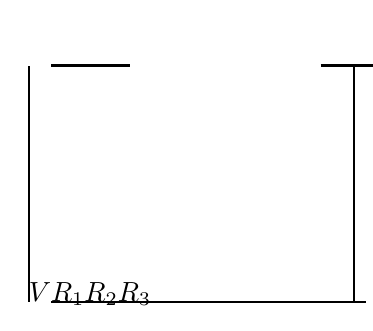
\begin{tikzpicture}[scale=1]
  \draw[thick] (0,0) -- (0,3);
  \generatore[rot=90, label=$V$, label dx=-0.7, label dy=0]{0}{1.5}{}
  \draw[thick] (0,0) -- (4,0);
  \draw[thick] (0,3) -- (1,3);
  \resistoreANSI[rot=0, label=$R_1$, label dy=0.5]{2}{3}{}
  \draw[thick] (3,3) -- (4,3);
  \draw[thick] (4,3) -- (4,2);
  \resistoreANSI[rot=90, label=$R_2$, label dx=0.5, label dy=0]{4}{1.5}{}
  \draw[thick] (4,1) -- (4,0);
  \draw[thick] (3,3) -- (3,0);
  \resistoreANSI[rot=90, label=$R_3$, label dx=0.5, label dy=0]{3}{1.5}{}
  \filldraw (3,3) circle (0.05) node[above] {A};
  \massa{3}{0}{}
\end{tikzpicture}
\end{center}

\textbf{Soluzione.} Scegliamo il nodo inferiore come riferimento (\(V = 0\)). Il nodo A ha potenziale \(V_A\) incognito. Applichiamo la LKC al nodo A:
\[
\frac{V - V_A}{R_1} = \frac{V_A}{R_2} + \frac{V_A}{R_3}.
\]
Da cui si ricava \(V_A\) e poi le correnti nei rami.
\end{esempio}

\section{Il teorema di Millman}

\begin{concetto}
Il \textbf{teorema di Millman} permette di calcolare la tensione ai capi di una rete formata da più rami in parallelo, ciascuno formato da un generatore di tensione in serie con un resistore. La tensione comune ai capi del parallelo è:
\[
V = \frac{\sum_k \frac{\mathcal{E}_k}{R_k}}{\sum_k \frac{1}{R_k}}.
\]
\end{concetto}

Il teorema di Millman è una conseguenza diretta del metodo dei potenziali ai nodi applicato a un circuito con un solo nodo indipendente.

\begin{esempio}
\textbf{Due generatori in parallelo.} Si considerino due generatori \(\mathcal{E}_1 = 12\,\text{V}\) con \(R_1 = 2\,\Omega\) e \(\mathcal{E}_2 = 6\,\text{V}\) con \(R_2 = 3\,\Omega\), collegati in parallelo. La tensione comune è:
\[
V = \frac{\frac{12}{2} + \frac{6}{3}}{\frac{1}{2} + \frac{1}{3}} = \frac{6 + 2}{0{,}5 + 0{,}333} = \frac{8}{0{,}833} = 9{,}6\,\text{V}.
\]
\end{esempio}

\section{Esercizi}

\subsection{Domande di comprensione}

\begin{enumerate}[leftmargin=1cm]
  \item Che cos'è una corrente di maglia? Perché non è una corrente fisica?
  \item In quali casi conviene usare il metodo delle correnti di maglia?
  \item Enuncia il principio di sovrapposizione degli effetti. Quali sono i limiti di validità?
  \item Che cosa significa ``spegnere un generatore''? Come si spegne un generatore di tensione? E uno di corrente?
  \item Enuncia il teorema di Thévenin e spiega come si calcolano \(V_{Th}\) e \(R_{Th}\).
  \item Enuncia il teorema di Norton. Che relazione c'è tra i parametri di Thévenin e quelli di Norton?
  \item In che cosa consiste il metodo dei potenziali ai nodi? Perché conviene scegliere un nodo di riferimento?
  \item Enuncia il teorema di Millman e spiega in quali circuiti si applica.
\end{enumerate}

\subsection{Esercizi sulle correnti di maglia}

\begin{esercizio}
\textbf{Esercizio svolto.} In un circuito con due maglie, le equazioni delle correnti di maglia sono:
\[
\begin{cases}
5 i_1 - 2 i_2 = 12 \\
-2 i_1 + 6 i_2 = -6
\end{cases}
\]
Calcolare \(i_1\) e \(i_2\).

\smallskip
\textbf{Soluzione.} Dalla prima equazione:
\[
i_1 = \frac{12 + 2 i_2}{5}.
\]
Sostituendo nella seconda:
\[
-2 \cdot \frac{12 + 2 i_2}{5} + 6 i_2 = -6.
\]
Moltiplicando per 5:
\[
-24 - 4 i_2 + 30 i_2 = -30 \quad\Rightarrow\quad 26 i_2 = -6 \quad\Rightarrow\quad i_2 = -\frac{3}{13} \approx -0{,}23\,\text{A}.
\]
\[
i_1 = \frac{12 + 2(-0{,}23)}{5} \approx 2{,}31\,\text{A}.
\]
\end{esercizio}

\textbf{Esercizi da svolgere.}
\begin{enumerate}[leftmargin=1cm]
  \item In un circuito a due maglie, le equazioni sono:
  \[
  \begin{cases}
  4 i_1 - i_2 = 10 \\
  -i_1 + 3 i_2 = 5
  \end{cases}
  \]
  Calcolare \(i_1\) e \(i_2\).
  \item In un circuito a due maglie, le equazioni sono:
  \[
  \begin{cases}
  6 i_1 - 2 i_2 = 18 \\
  -2 i_1 + 5 i_2 = -8
  \end{cases}
  \]
  Calcolare \(i_1\) e \(i_2\).
  \item In un circuito a tre maglie, le equazioni sono:
  \[
  \begin{cases}
  3 i_1 - i_2 = 6 \\
  -i_1 + 4 i_2 - i_3 = 0 \\
  -i_2 + 2 i_3 = -3
  \end{cases}
  \]
  Calcolare \(i_1\), \(i_2\) e \(i_3\).
\end{enumerate}

\subsection{Esercizi sulla sovrapposizione degli effetti}

\begin{esercizio}
\textbf{Esercizio svolto.} Un circuito è formato da due generatori \(\mathcal{E}_1 = 6\,\text{V}\) e \(\mathcal{E}_2 = 3\,\text{V}\) e due resistori \(R_1 = 2\,\Omega\) e \(R_2 = 4\,\Omega\) in serie. Calcolare la corrente usando la sovrapposizione degli effetti.

\smallskip
\textbf{Soluzione.} Con \(\mathcal{E}_2\) spento (cortocircuito):
\[
I' = \frac{\mathcal{E}_1}{R_1 + R_2} = \frac{6}{6} = 1\,\text{A}.
\]
Con \(\mathcal{E}_1\) spento:
\[
I'' = \frac{\mathcal{E}_2}{R_1 + R_2} = \frac{3}{6} = 0{,}5\,\text{A}.
\]
Se i due generatori sono concordi, la corrente totale è \(I = I' + I'' = 1{,}5\,\text{A}\).
\end{esercizio}

\textbf{Esercizi da svolgere.}
\begin{enumerate}[leftmargin=1cm]
  \item Un circuito ha due generatori \(\mathcal{E}_1 = 9\,\text{V}\) e \(\mathcal{E}_2 = 3\,\text{V}\) e un resistore \(R = 3\,\Omega\). Calcolare la corrente usando la sovrapposizione.
  \item Un circuito ha due generatori in parallelo: \(\mathcal{E}_1 = 12\,\text{V}\) con \(R_1 = 4\,\Omega\) e \(\mathcal{E}_2 = 6\,\text{V}\) con \(R_2 = 2\,\Omega\). Calcolare la corrente in ciascun ramo usando la sovrapposizione.
\end{enumerate}

\subsection{Esercizi su Thévenin e Norton}

\begin{esercizio}
\textbf{Esercizio svolto.} Un circuito è formato da un generatore \(V = 10\,\text{V}\) e due resistori \(R_1 = 5\,\Omega\) e \(R_2 = 5\,\Omega\) in serie. Calcolare il circuito equivalente di Thévenin visto ai capi di \(R_2\).

\smallskip
\textbf{Soluzione.} \(V_{Th}\) è la tensione a vuoto ai capi di \(R_2\):
\[
V_{Th} = V \frac{R_2}{R_1 + R_2} = 10 \cdot \frac{5}{10} = 5\,\text{V}.
\]
\(R_{Th}\) è la resistenza vista dai terminali con il generatore spento:
\[
R_{Th} = R_1 \parallel R_2 = \frac{5 \cdot 5}{5+5} = 2{,}5\,\Omega.
\]
Il circuito equivalente di Thévenin è un generatore da \(5\,\text{V}\) in serie con \(2{,}5\,\Omega\).
\end{esercizio}

\textbf{Esercizi da svolgere.}
\begin{enumerate}[leftmargin=1cm]
  \item Un circuito è formato da \(V = 24\,\text{V}\), \(R_1 = 6\,\Omega\) e \(R_2 = 3\,\Omega\) in serie. Calcolare il circuito equivalente di Thévenin visto ai capi di \(R_2\).
  \item Un circuito è formato da \(V = 9\,\text{V}\), \(R_1 = 1\,\text{k}\Omega\) e \(R_2 = 2\,\text{k}\Omega\) in serie. Calcolare il circuito equivalente di Thévenin e di Norton visto ai capi di \(R_2\).
  \item Dato il circuito equivalente di Thévenin con \(V_{Th} = 6\,\text{V}\) e \(R_{Th} = 3\,\Omega\), calcolare i parametri del circuito equivalente di Norton.
\end{enumerate}

\subsection{Esercizi sui potenziali ai nodi e Millman}

\begin{esercizio}
\textbf{Esercizio svolto.} Un circuito ha un nodo A collegato a massa tramite \(R_1 = 2\,\Omega\), a un generatore \(V = 12\,\text{V}\) tramite \(R_2 = 4\,\Omega\), e a un altro generatore \(V_2 = 6\,\text{V}\) tramite \(R_3 = 3\,\Omega\). Calcolare il potenziale del nodo A.

\smallskip
\textbf{Soluzione.} Applichiamo Millman:
\[
V_A = \frac{\frac{12}{4} + \frac{6}{3}}{\frac{1}{2} + \frac{1}{4} + \frac{1}{3}} = \frac{3 + 2}{0{,}5 + 0{,}25 + 0{,}333} = \frac{5}{1{,}083} \approx 4{,}62\,\text{V}.
\]
\end{esercizio}

\textbf{Esercizi da svolgere.}
\begin{enumerate}[leftmargin=1cm]
  \item Un circuito ha due generatori in parallelo: \(\mathcal{E}_1 = 10\,\text{V}\) con \(R_1 = 2\,\Omega\) e \(\mathcal{E}_2 = 5\,\text{V}\) con \(R_2 = 3\,\Omega\). Calcolare la tensione comune usando Millman.
  \item Tre rami in parallelo hanno: \(\mathcal{E}_1 = 12\,\text{V}\), \(R_1 = 4\,\Omega\); \(\mathcal{E}_2 = 6\,\text{V}\), \(R_2 = 2\,\Omega\); \(\mathcal{E}_3 = 3\,\text{V}\), \(R_3 = 1\,\Omega\). Calcolare la tensione comune.
  \item Un circuito ha un nodo A con tre resistori collegati a massa: \(R_1 = 1\,\Omega\), \(R_2 = 2\,\Omega\), \(R_3 = 3\,\Omega\), e un generatore \(V = 12\,\text{V}\) collegato tramite \(R_4 = 4\,\Omega\). Calcolare il potenziale del nodo A.
\end{enumerate}